\begin{figure}

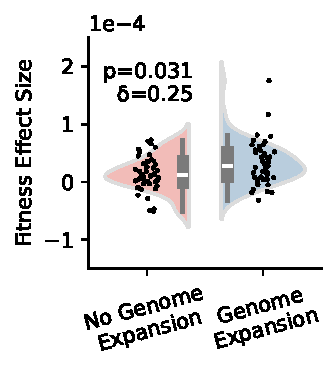
\includegraphics[width=0.39\linewidth]{%
binder-2025-09-05-genome-expansion-fitness/binder/teeplots/2025-09-05-genome-expansion-fitness/biotic_background=Contemporary+hue=genome-expansion+palette=pastel1+subject=Population+test=mw+viz=violinplot+x=genome-expansion+y=fitness-differential-focal+ext=.pdf}
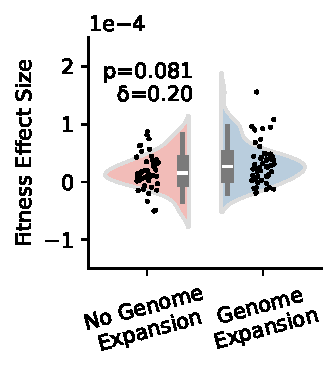
\includegraphics[width=0.305\linewidth, trim={1.3cm 0 0 0.6cm}, clip]{%
binder-2025-09-05-genome-expansion-fitness/binder/teeplots/2025-09-05-genome-expansion-fitness/biotic_background=Prefatory+hue=genome-expansion+palette=pastel1+subject=Population+test=mw+viz=violinplot+x=genome-expansion+y=fitness-differential-focal+ext=.pdf}%
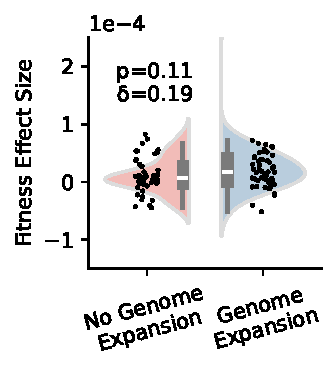
\includegraphics[width=0.305\linewidth, trim={1.3cm 0 0 0.6cm}, clip]{%
binder-2025-09-05-genome-expansion-fitness/binder/teeplots/2025-09-05-genome-expansion-fitness/biotic_background=Without+hue=genome-expansion+palette=pastel1+subject=Population+test=mw+viz=violinplot+x=genome-expansion+y=fitness-differential-focal+ext=.pdf}

\vspace{-1ex}

\begin{subfigure}{0.135\linewidth}
~
\end{subfigure}%
\begin{subfigure}{0.305\linewidth}
    \centering
    \caption{\footnotesize contemporary\\background}
    \label{fig:genome-expansion-population:contemporary}
\end{subfigure}%
\begin{subfigure}{0.305\linewidth}
    \centering
    \caption{\footnotesize prefatory\\background}
    \label{fig:genome-expansion-population:prefatory}
\end{subfigure}%
\begin{subfigure}{0.255\linewidth}
    \centering
    \caption{\footnotesize without\\background}
    \label{fig:genome-expansion-population:without}
\end{subfigure}



\caption{
    \textbf{Co-occurence of adaptation with genome expansion, population fitness assays.}
    \footnotesize
    Violin plots compare adaptation assay outcome distributions between focal specimens with genome size increase relative to ancestor and those without.
    Assays compete focal population at stint $n+1$ against focal population at stint $n$;
    panels report outcomes under three assay designs, differing in biotic context.
    When competed in the presence of background strain population from stint $n+1$, stronger adaptation accompanies genome expansions --- with small effect size (panel \ref{fig:genome-expansion-population:contemporary}; $p = 0.031, \; \delta = 0.25$).
    When competed with no biotic background, similar trends appear with small effect size under fitness assays both with prefatory (stint $n$) biotic background and without biotic background --- although not significant under a two-tailed alternative hypothesis (panels \labelcref{fig:genome-expansion-population:prefatory,fig:genome-expansion-population:without}; $p=0.08,\; 0.11; \; \delta = 0.20, \; 0.19$).
    Reported statistics are Cliff's delta, a non-parametric effect size metric ranging from 0.0 to 1.0, and two-tailed Mann-Whitney U test; significance testing with two-sample $t$-tests (two-tailed alternative) gave similar results.
    Figure \ref{fig:genome-expansion-population} reports analyses using specimen adaptation assays.
}
\label{fig:genome-expansion-population}

\end{figure}
